\documentclass{AISB2008}
\usepackage{newfloat}
\DeclareFloatingEnvironment[fileext=frm,placement={!ht},name=Listing]{listing}
\usepackage{placeins}
\usepackage{listings}


\lstset{
  xleftmargin=.35\columnwidth, xrightmargin=.35\columnwidth
}

\usepackage{times}
\usepackage{graphicx}
\usepackage{latexsym}

\usepackage{amsmath}

\makeatletter
\renewcommand{\boxed}[1]{\text{\fboxsep=.2em\fbox{\m@th$\displaystyle#1$}}}
\makeatother

\newcommand{\mystrut}{\vphantom{b\gamma}}

\usepackage{amsopn}
\newcommand{\droparrow}{%
  \mathchoice{\raisebox{-4pt}{$\displaystyle\mapsto$}}
             {\raisebox{-4pt}{$\mapsto$}}
             {\raisebox{-2pt}{$\scriptstyle\mapsto$}}
             {\raisebox{-2pt}{$\scriptscriptstyle\mapsto$}}}

\usepackage{marvosym,hetcasl}


\usepackage[hidelinks]{hyperref}

\begin{document}

\title{The Search for Computational Intelligence}

\author{Joseph Corneli%
\institute{Department of Computing, Goldsmiths College, University of London\newline
\Email \url{j.corneli@gold.ac.uk}}%
\and%
Ewen Maclean%
\institute{School of Informatics, University of Edinburgh\newline
\Email \url{ewenmaclean@gmail.com}}}

\maketitle
\bibliographystyle{AISB2008}

\begin{abstract}
XXX YYY
\end{abstract}

\section{Introduction}

\begin{figure}
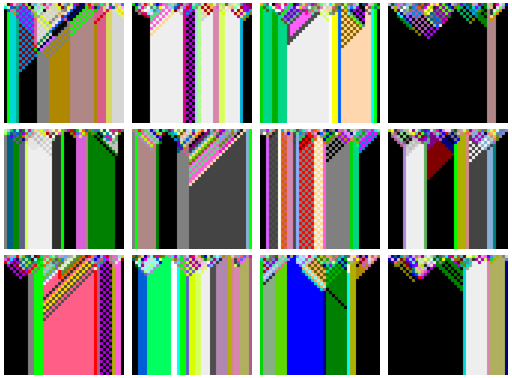
\includegraphics[width=\columnwidth]{metaca.png}
\caption{An illustration of MetaCA evolution\label{metaca-taster}}
\end{figure}

This paper takes a local approach to studying the
evolution of cellular automata, following on the
global approach of \cite{pavlic2014self}.

\newpage

\section{Background}

\subsection{Cellular Automata}

\cite{mitchell1993revisiting} is the classic work on ``edge of
chaos.'' (Read more here and talk about the $\lambda$ thing.)

\cite{hofstadter1995prolegomena,marshall1999metacat} took a rather
different but still somewhat related approach.


Explain the background on computational blending and why we thought
domain would be a revealing experiment.  (Basically, CAs do a simple
kind of blending already.)

\subsection{Conceptual Blending}

Following the approach of Goguen \cite{}, we propose exploiting
existing formalisms of blending in the context of cellular automata to
investigate emergent and novel behaviours. The fundamental building blocks used in calculating concept or theory blends are
\begin{description}
\item[Input Concepts] are the theories or concepts which have some degree of commonality, which is not necessarily syntactic. 
\item[Signature Morphism] is a definition of how symbols are mapped between theories or concepts. 
\item[Generic Space] is the space which contains a theory which is common to both input theories.
\item[Blend] is the space computed by combining both theories. The computation is computed using a ``pushout'' from the underlying categorical semantics \cite{}. 
\end{description}

Once a blend has been computed, it may represent a concept which is in some way inconsistent. Equally it may represent a concept which is in some way incomplete. We can then either weaken an input teory or refine the blend:
\begin{description}
\item[Weakening] Given an inconsistent blend it is possible to weaken the input concept in order to produce a consistent blend. Weakening means removing symbols or axioms from the input concept.
\item[Refinement] Given a blend which represents a concept which is in some way incomplete, it is possible to refine the concept by adding symbols or axioms.
\end{description}

This paper presents an example of concepts to which the blending
process applies.  We describe the components of blending in the
context of cellular automata in Sections \ref{introducing-blending}
and \ref{2d-experiments-design}.

\clearpage

\section{Implementation}
%%%% describe genotype/phenotype definition?


%%%% section header?
\subsection{Generating Genotypes}

To explain how this works, consider the following example.  Each
elementary CA rule defines a mapping from all eight strings of 0's and
1's to the set \{0,1\}.  Thus, for example the rule 01010100 is defined as the following operation:
\begin{lstlisting}[mathescape]
0 0 0 $\mapsto$ 0
0 0 1 $\mapsto$ 1
0 1 0 $\mapsto$ 0
0 1 1 $\mapsto$ 1
1 0 0 $\mapsto$ 0
1 0 1 $\mapsto$ 1
1 1 0 $\mapsto$ 0
1 1 1 $\mapsto$ 0
\end{lstlisting}
%  $\text{\emph{Rule 84}}$ 
%  ... Must double check the example, since I had a mistake in the truth table

There are 256 of these rules; the example above is Rule 84 in
Wolfram's numbering \cite{wolfram1994cellular}.  The basic concept of
the MetaCA is to evolve a CA with 256 possible states -- rather than
the traditional 2 -- where state now corresponds to a ``CA rule''.
Then we can then apply this rule to decide the output for the next
cell, depending also on the state of the neighbouring cells.  By
positioning three CA rules next to each other, we define a
multiplication by applying the central rule bitwise across the alleles.
%
For example, here is the result of multiplying $01101110\times
01010100\times 01010101$.  In the context of such a multiplication, we
refer to the central multiplicand as the ``local rule,'' and we
highlight it in bold below.

\lstset{
  xleftmargin=.1\columnwidth, xrightmargin=.01\columnwidth
}

\begin{lstlisting}[mathescape]
0 $\mathbf{0}$ 0     $0$     $\text{\emph{Apply local rule to ``000''}}$
1 $\mathbf{1}$ 1     $0$     $\text{\emph{Apply local rule to ``111}}$
1 $\mathbf{0}$ 0     $0$     $\text{\emph{Apply local rule to ``100''}}$
0 $\mathbf{1}$ 1  $\droparrow$   $1$     $\text{\emph{Apply local rule to ``011''}}$
1 $\mathbf{0}$ 0     $0$     $\text{\emph{Apply local rule to ``100''}}$
1 $\mathbf{1}$ 1     $0$     $\text{\emph{Apply local rule to ``111''}}$
1 $\mathbf{0}$ 0     $0$     $\text{\emph{Apply local rule to ``100''}}$
0 $\mathbf{0}$ 1     $1$     $\text{\emph{Apply local rule to ``001''}}$
\end{lstlisting}

Realised in a simulation, the results are not particularly impressive:
they stabilise early and do not produce any interesting patterns
(Figure \ref{barcode}).

\begin{figure}
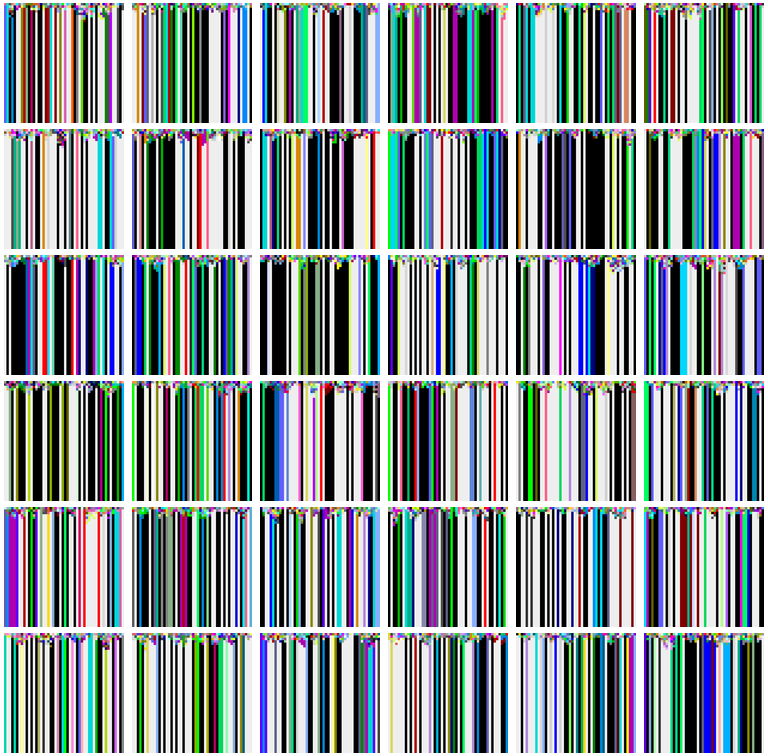
\includegraphics[width=\columnwidth,trim = 135mm 177mm 0mm 0mm,clip=true]{paint-drips.png}
\caption{Under evolution according to the local rule without blending
  dynamics, a barcode-like stable pattern forms
  quickly\label{barcode}}
\end{figure}

%%%introduce blending
\subsection{Introducing Blending} \label{introducing-blending}

%%% say what the input concepts are - call them input rules

The blending variant says to first compute the ``generic space'' by
noting the alleles where the two adjacent neighbours are the same, and
where they differ.  Only when the generic space retains some ambiguity
(indicated by $\{0,1\}$), we apply the local rule (again recorded on
the centre cell at left and highlighted in bold) in a bitwise manner
across each allele, to arrive at the final result.

\lstset{
  xleftmargin=.05\columnwidth, xrightmargin=.01\columnwidth
}

\begin{lstlisting}[mathescape]
0 $\mathbf{0}$ 0       0       $\:0$    $\text{\emph{Neighbours are both 0}}$
1 $\mathbf{1}$ 1       1       $\:1$    $\text{\emph{Neighbours are both 1}}$
1 $\mathbf{0}$ 0     {0,1}     $\boxed{0}$    $\text{\emph{Apply local rule to ``100''}}$
0 $\mathbf{1}$ 1  $\droparrow$   {0,1}  $\droparrow$   $\boxed{1}$    $\text{\emph{Apply local rule to ``011''}}$
1 $\mathbf{0}$ 0     {0,1}     $\boxed{0}$    $\text{\emph{Apply local rule to ``100''}}$
1 $\mathbf{1}$ 1       1       $\:1$    $\text{\emph{Neighbours are both 1}}$
1 $\mathbf{0}$ 0     {0,1}     $\boxed{0}$    $\text{\emph{Apply local rule to ``100''}}$
0 $\mathbf{0}$ 1     {0,1}     $\boxed{1}$    $\text{\emph{Apply local rule to ``001''}}$
\end{lstlisting}

For illustrative purposes, this blend has been formalised in the HETS
system \cite{mossakowski2007heterogeneous} by introducing CASL files
to represent the 8 bit encodings (Listing \ref{CASL-listing}).
%
The computed blend is inconsistent as there is not a unique value
representing the output value of each function.  In order to resolve
this we weaken the input rules in CASL by removing the function values
which cause conflict.
%
Note that purposes of efficiency, we have implemented our 1D
experiments in LISP rather than in \mbox{HETS}/\mbox{CASL}.  We've put
the working code on
Github\footnote{\url{https://github.com/holtzermann17/metaca}}.

%%%% the CASL latex is now in a Listing environment below

\subsection{2D Experiments} \label{2d-experiments-design}

We've developed a parallel implementation in the 2D case, inspired by
Conway's Game of Life.  Conway's rule says that a cell dies when less
than 3 or more than 5 of its 8 neighbours (in cardinal and
intercardinal directions) are alive, survives when 3, 4, or 5
neighbours are alive, and that it reproduces when 3 or 4 neighbours
are alive.  This standard case is illustrated in Figure
\ref{conway-rule}.

\begin{figure}[!ht]
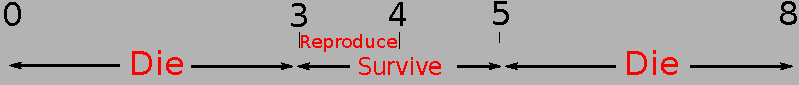
\includegraphics[width=\columnwidth]{conway}
\caption{Conway rule for the Game of Life\label{conway-rule}}
\end{figure}

We've considered generalisations variants of this rule (Figure
\ref{generalised-conway-rule}), giving each cell a \emph{weight}
(between 0 and 1000) and a genotype that sets the survival parameters
$x$, $y$, and $z$ in terms of the sum of weights of the neighours.
\begin{figure}[!ht]
\includegraphics[width=\columnwidth]{2dgenotype}
\caption{Generalisation of Conway's rule\label{generalised-conway-rule}}
\end{figure}

These genotypes can also be blended: given two genotypes $(x_1, y_1,
z_1)$ and $(x_2, y_2, z_2)$, the blend is $(\mathrm{min} \{x_1,x_2\},
\mathrm{max} \{y_1,y_2\}, \mathrm{max} \{z_1,z_2\})$; see Figure
\ref{blending-2d-rule}.  This blend corresponds to \textbf{[\ldots
    Ewen please add a line or so here]}.

The 2D simulations have been realised in an interactive Java
applet\footnote{\url{http://www.algorhythmical.co.uk/cablender.html}}
and the code is available\footnote{Where?}.

\FloatBarrier
\newpage

\begin{listing}
{\scriptsize
\begin{hetcasl}
\KW{library} \Id{metaca}\\
\\
\KW{logic} \SId{CASL}\\
\\
\SPEC \=\SIdIndex{METACABitencoding} \Ax{=}\\
\> \KW{free} \KW{type} \=\Id{Bit} \Ax{:}\Ax{:}\=\Ax{=} \Ax{0} \AltBar{} \Ax{1}\\
\> \SORT \Id{Triple}\\
\> \OPS \=\Id{t} \Ax{:} \=\Id{Bit} \Ax{\times} \Id{Bit} \Ax{\times} \Id{Bit} \Ax{\rightarrow} \Id{Triple};\\
\>\> \Id{bitop}\Ax{\_\_} \Ax{:} \=\Id{Triple} \Ax{\rightarrow} \Id{Bit}\\
\KW{end}\\
\\
\SPEC \=\SIdIndex{LeftRule} \Ax{=}\\
\> \SId{METACABitencoding}\\
\THEN \=\Ax{\bullet} \=\Id{bitop} \Id{t}(\=\Ax{0}, \Ax{0}, \Ax{0}) \Ax{=} \Ax{0}\\
\> \Ax{\bullet} \=\Id{bitop} \Id{t}(\=\Ax{0}, \Ax{0}, \Ax{1}) \Ax{=} \Ax{1}\\
\> \Ax{\bullet} \=\Id{bitop} \Id{t}(\=\Ax{0}, \Ax{1}, \Ax{0}) \Ax{=} \Ax{1}\\
\> \Ax{\bullet} \=\Id{bitop} \Id{t}(\=\Ax{0}, \Ax{1}, \Ax{1}) \Ax{=} \Ax{0}\\
\> \Ax{\bullet} \=\Id{bitop} \Id{t}(\=\Ax{1}, \Ax{0}, \Ax{0}) \Ax{=} \Ax{1}\\
\> \Ax{\bullet} \=\Id{bitop} \Id{t}(\=\Ax{1}, \Ax{0}, \Ax{1}) \Ax{=} \Ax{1}\\
\> \Ax{\bullet} \=\Id{bitop} \Id{t}(\=\Ax{1}, \Ax{1}, \Ax{0}) \Ax{=} \Ax{1}\\
\> \Ax{\bullet} \=\Id{bitop} \Id{t}(\=\Ax{1}, \Ax{1}, \Ax{1}) \Ax{=} \Ax{0}\\
\KW{end}\\
\\
\SPEC \=\SIdIndex{RightRule} \Ax{=}\\
\> \SId{METACABitencoding}\\
\THEN \=\Ax{\bullet} \=\Id{bitop} \Id{t}(\=\Ax{0}, \Ax{0}, \Ax{0}) \Ax{=} \Ax{0}\\
\> \Ax{\bullet} \=\Id{bitop} \Id{t}(\=\Ax{0}, \Ax{0}, \Ax{1}) \Ax{=} \Ax{1}\\
\> \Ax{\bullet} \=\Id{bitop} \Id{t}(\=\Ax{0}, \Ax{1}, \Ax{0}) \Ax{=} \Ax{0}\\
\> \Ax{\bullet} \=\Id{bitop} \Id{t}(\=\Ax{0}, \Ax{1}, \Ax{1}) \Ax{=} \Ax{1}\\
\> \Ax{\bullet} \=\Id{bitop} \Id{t}(\=\Ax{1}, \Ax{0}, \Ax{0}) \Ax{=} \Ax{0}\\
\> \Ax{\bullet} \=\Id{bitop} \Id{t}(\=\Ax{1}, \Ax{0}, \Ax{1}) \Ax{=} \Ax{1}\\
\> \Ax{\bullet} \=\Id{bitop} \Id{t}(\=\Ax{1}, \Ax{1}, \Ax{0}) \Ax{=} \Ax{0}\\
\> \Ax{\bullet} \=\Id{bitop} \Id{t}(\=\Ax{1}, \Ax{1}, \Ax{1}) \Ax{=} \Ax{1}\\
\KW{end}\\
\\
\SPEC \=\SIdIndex{LocalRule} \Ax{=}\\
\> \SId{METACABitencoding}\\
\THEN \=\Ax{\bullet} \=\Id{bitop} \Id{t}(\=\Ax{0}, \Ax{0}, \Ax{0}) \Ax{=} \Ax{0}\\
\> \Ax{\bullet} \=\Id{bitop} \Id{t}(\=\Ax{0}, \Ax{0}, \Ax{1}) \Ax{=} \Ax{1}\\
\> \Ax{\bullet} \=\Id{bitop} \Id{t}(\=\Ax{0}, \Ax{1}, \Ax{0}) \Ax{=} \Ax{0}\\
\> \Ax{\bullet} \=\Id{bitop} \Id{t}(\=\Ax{0}, \Ax{1}, \Ax{1}) \Ax{=} \Ax{1}\\
\> \Ax{\bullet} \=\Id{bitop} \Id{t}(\=\Ax{1}, \Ax{0}, \Ax{0}) \Ax{=} \Ax{0}\\
\> \Ax{\bullet} \=\Id{bitop} \Id{t}(\=\Ax{1}, \Ax{0}, \Ax{1}) \Ax{=} \Ax{1}\\
\> \Ax{\bullet} \=\Id{bitop} \Id{t}(\=\Ax{1}, \Ax{1}, \Ax{0}) \Ax{=} \Ax{0}\\
\> \Ax{\bullet} \=\Id{bitop} \Id{t}(\=\Ax{1}, \Ax{1}, \Ax{1}) \Ax{=} \Ax{0}\\
\KW{end}\\
\\
\SPEC \=\SIdIndex{Generic} \Ax{=}\\
\> \SId{METACABitencoding}\\
\THEN \=\Ax{\bullet} \=\Id{bitop} \Id{t}(\=\Ax{0}, \Ax{0}, \Ax{0}) \Ax{=} \Ax{0}\\
\> \Ax{\bullet} \=\Id{bitop} \Id{t}(\=\Ax{0}, \Ax{0}, \Ax{1}) \Ax{=} \Ax{1}\\
\> \Ax{\bullet} \=\Id{bitop} \Id{t}(\=\Ax{1}, \Ax{0}, \Ax{1}) \Ax{=} \Ax{1}\\
\KW{end}\\
\\
\VIEW \=\SId{Left} \Ax{:} \=\SId{Generic} \KW{to} \SId{LeftRule}\\
\KW{end}\\
\\
\VIEW \=\SId{Right} \Ax{:} \=\SId{Generic} \KW{to} \SId{RightRule}\\
\KW{end}\\
\\
\SPEC \=\SIdIndex{Blend} \Ax{=}\\
\> \KW{combine} \=\Id{Left}, \Id{Right}\\
\KW{end}\\
\\
\SPEC \=\SIdIndex{WeakenedLeftRule} \Ax{=}\\
\> \SId{METACABitencoding}\\
\THEN \=\Ax{\bullet} \=\Id{bitop} \Id{t}(\=\Ax{0}, \Ax{0}, \Ax{0}) \Ax{=} \Ax{0}\\
\> \Ax{\bullet} \=\Id{bitop} \Id{t}(\=\Ax{0}, \Ax{0}, \Ax{1}) \Ax{=} \Ax{1}\\
\> \Ax{\bullet} \=\Id{bitop} \Id{t}(\=\Ax{0}, \Ax{1}, \Ax{0}) \Ax{=} \Ax{1}\\
\> \Ax{\bullet} \=\Id{bitop} \Id{t}(\=\Ax{0}, \Ax{1}, \Ax{1}) \Ax{=} \Ax{0}\\
\> \Ax{\bullet} \=\Id{bitop} \Id{t}(\=\Ax{1}, \Ax{0}, \Ax{0}) \Ax{=} \Ax{1}\\
\> \Ax{\bullet} \=\Id{bitop} \Id{t}(\=\Ax{1}, \Ax{0}, \Ax{1}) \Ax{=} \Ax{1}\\
\> \Ax{\bullet} \=\Id{bitop} \Id{t}(\=\Ax{1}, \Ax{1}, \Ax{0}) \Ax{=} \Ax{1}\\
\KW{end}\\
\\
\SPEC \=\SIdIndex{WeakenedRightRule} \Ax{=}\\
\> \SId{METACABitencoding}\\
\THEN \=\Ax{\bullet} \=\Id{bitop} \Id{t}(\=\Ax{0}, \Ax{0}, \Ax{0}) \Ax{=} \Ax{0}\\
\> \Ax{\bullet} \=\Id{bitop} \Id{t}(\=\Ax{0}, \Ax{0}, \Ax{1}) \Ax{=} \Ax{1}\\
\> \Ax{\bullet} \=\Id{bitop} \Id{t}(\=\Ax{1}, \Ax{0}, \Ax{1}) \Ax{=} \Ax{1}\\
\> \Ax{\bullet} \=\Id{bitop} \Id{t}(\=\Ax{1}, \Ax{1}, \Ax{1}) \Ax{=} \Ax{1}\\
\KW{end}\\
\\
\VIEW \=\SId{WeakenedLeft} \Ax{:} \=\SId{Generic} \KW{to} \SId{WeakenedLeftRule}\\
\KW{end}\\
\\
\VIEW \=\SId{WeakenedRight} \Ax{:} \=\SId{Generic} \KW{to} \SId{WeakenedRightRule}\\
\KW{end}\\
\\
\SPEC \=\SIdIndex{ConsistentBlend} \Ax{=}\\
\> \KW{combine} \=\Id{WeakenedLeft}, \Id{WeakenedRight}\\
\KW{end}
\end{hetcasl}}
\caption{CASL source code listing calculating the running example $01101110\times 01010100\times 01010101$ via the blending meta-rule\label{CASL-listing}}
\end{listing}

\newpage

\begin{figure}[!ht]
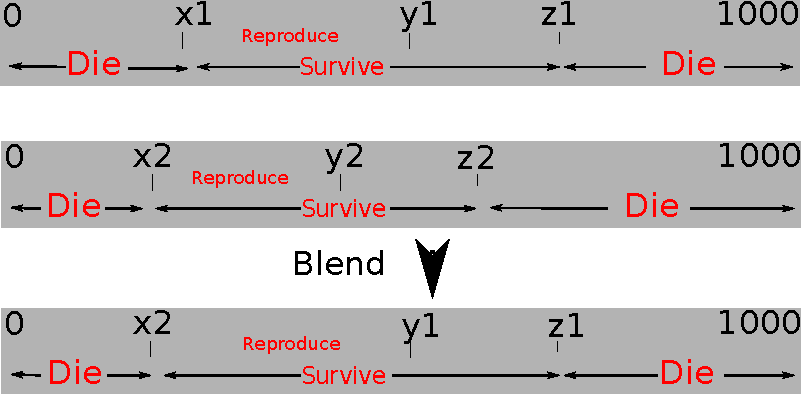
\includegraphics[width=\columnwidth]{2dgenotypeblend}
\caption{Defining blending dynamics for 2D genotypes\label{blending-2d-rule}}
\end{figure}

% \clearpage

\section{Results}
\subsection{1D CAs} \label{1d-results}

One of the first things we noticed was that even though the blending
dynamic creates more interesting ``CA-like'' patterns than simple
evolution according to the local rule (as illustrated in Figure
\ref{metaca-taster}), it also forms stable bands after this
interesting initial period.  In Figure \ref{flag}, this is illustrated
in a CA running with 500 cells over 500 generations.  Figure
\ref{flag} also includes a phenotype (in black and white) which is
driven entirely by the genotype: that is, if the local genotype is
\boxed{\alpha\mystrut}\boxed{\beta\mystrut}\boxed{\gamma\mystrut} 
where $\alpha, \beta, \gamma \in \{0,1\}^8$
and the local phenotype is
%
\boxed{a\mystrut}\boxed{b\mystrut}\boxed{c\mystrut}
where $a, b, c \in \{0,1\}$
%
then the genotype evolves locally according to the meta-rule $\alpha
\times \beta \times \gamma$ (in the blending variant described above)
while the phenotype evolves by applying the local rule $\beta$ to the
data ``$abc$.''

\begin{figure}

\includegraphics[width=\columnwidth]{flag.png}
\caption{Phenotype with behaviour determined by genotype\label{flag}}
\end{figure}

In the phenotype layer, we see a few bands with interesting patterns,
where the MetaCA at left has stabilised locally into one of the more
interesting CA rules.  However, the long term evolution is not
particularly interesting.  

We therefore decided to introduce random mutations to the genotype,
illustrated in Figures \ref{random-mutation}--\ref{seti}.  With a high
mutation rate, both genotype and phenotype are almost reduced to
confetti.  If we reduce the mutation rate sufficiently, some degree of
stability is preserved, and the vertically striped bands are
transformed into intermingling swaths of colour (Figure
\ref{lower-rate}).  We also see areas with more finely-grained
structure in the phenotype layer.  

In Figure \ref{seti}, the colour-coded genotype layer has been
replaced with a greyscale coding, and we see more clearly how the
phenotype behaviour follows that of the genotype.  That is, genotypes
similar to Rule 0 (00000000) or Rule 256 (11111111) tend to produce 0
or 1, respectively, in the phenotype layer.  Rules that output a blend
of 0's and 1's are mapped to grey shades.  Several interesting rules
(Rule 110, Rule 30, Rule 90, Rule 184, and their reversals, bitwise
inverses, and inverted-reversals) are highlighted in colour.  In
particular, Rule 110 variants are highlighted in red.

%% \begin{figure}
%% 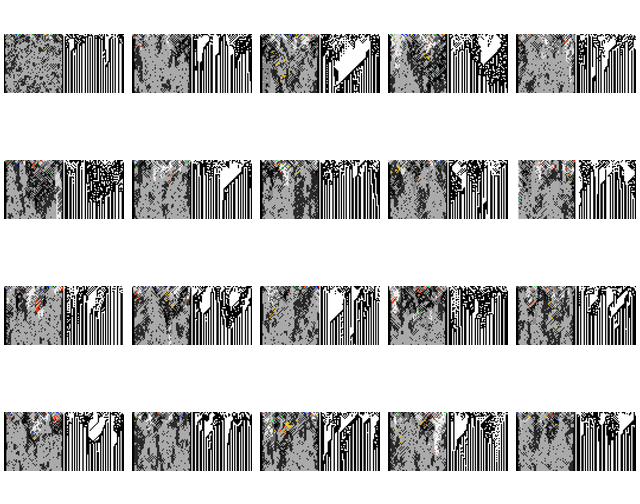
\includegraphics[width=\columnwidth]{baldwin.png}
%% \caption{Introducing a Baldwin effect}
%% \end{figure}

\begin{figure}
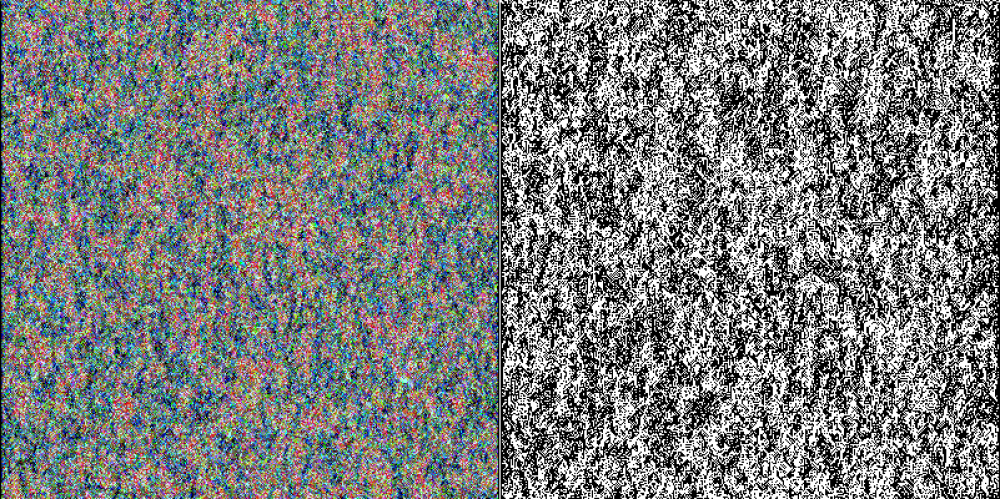
\includegraphics[width=\columnwidth]{big.png}
\caption{A high rate of mutation produces tantalising random structures \label{random-mutation}}
\end{figure}

\begin{figure}
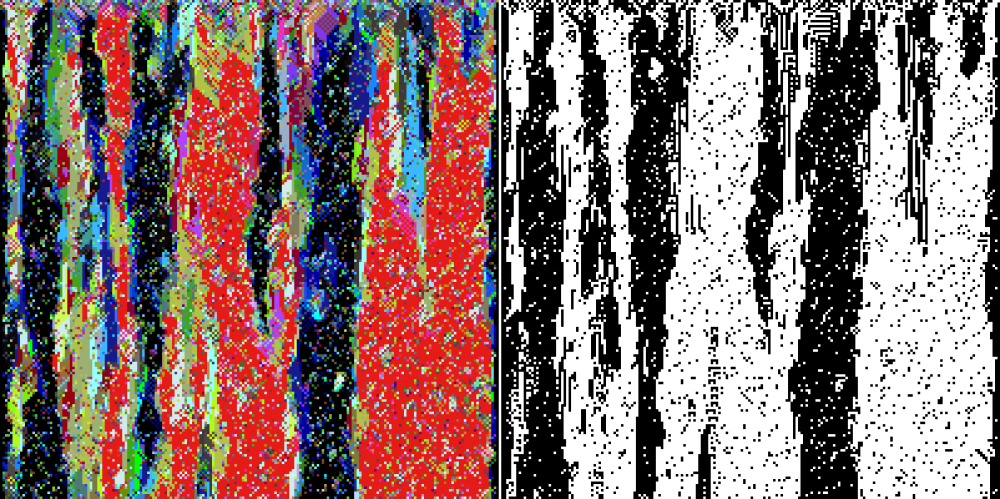
\includegraphics[width=\columnwidth]{lamp-down-low.png}
\caption{Throttling down the mutation rate preserves some of the large-scale stability while making room for variability \label{lower-rate}}
\end{figure}

\begin{figure}
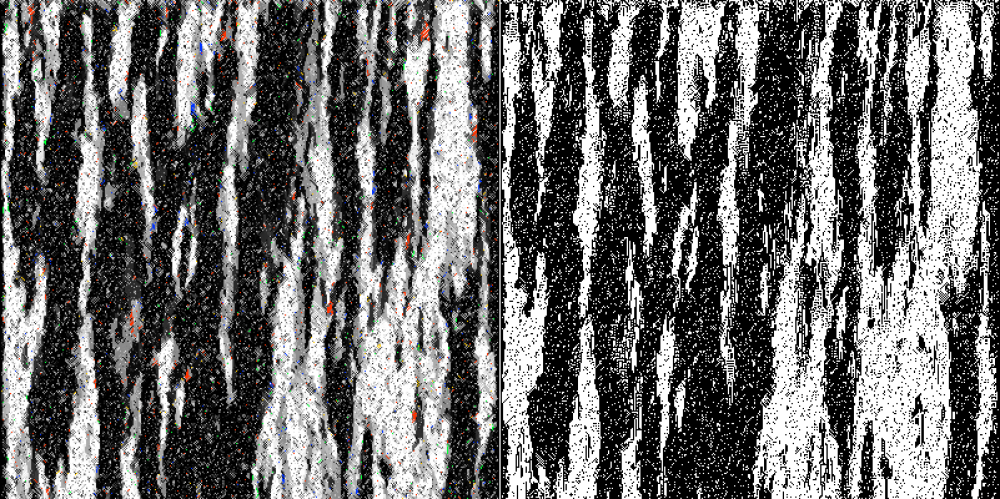
\includegraphics[width=\columnwidth]{seti.png}
\caption{The search for intelligent life in the computational universe \label{seti}}
\end{figure}

We observe that Rule 0 and Rule 256-like behaviour tends to
predominate.  Grey areas appear to be semi-stable.  Red patches appear
and disappear, as if independent planets evolve intelligent life and
are then extinguished.  With this physics, ``intelligent life'' seems
inevitable, but also inevitably short-lived.  One would have to look
for another overall physics for intelligent behaviour to predominate.

A potential indication of the direction to look in is presented in
Figure \ref{reef}, which presents CAs generated by adjusting the
typical blending evolution pattern by an (erroneously-programmed)
mutation rule that only flips the first bit.  We see that long-term
behaviour in the genotype flutters randomly between Rule 0 (00000000)
and Rule 128 (10000000).  The short-term behaviour in the phenotype is
nevertheless quite interesting, exhibiting many of the familiar
lifelike edge-of-chaos patterns before ultimately succombing to a
version of Newton's First Law.

\begin{figure}
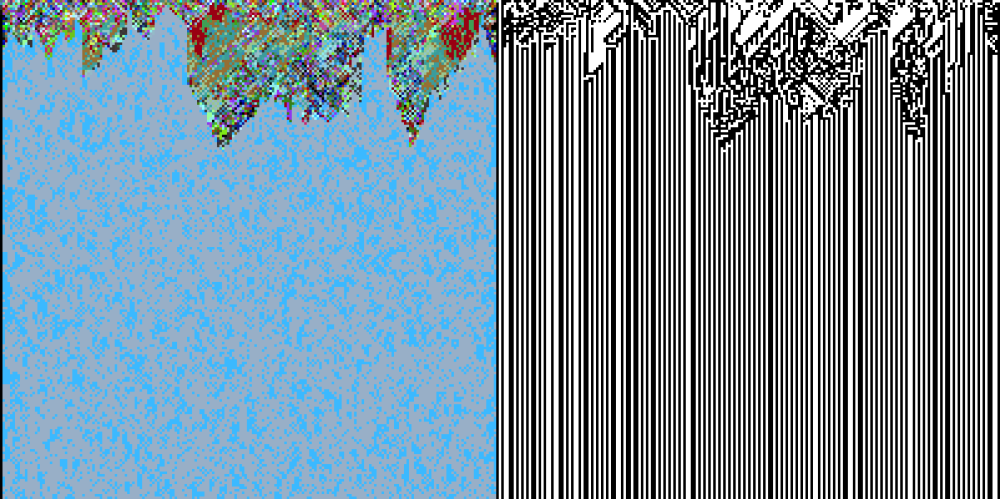
\includegraphics[width=\columnwidth]{reef.png} \newline
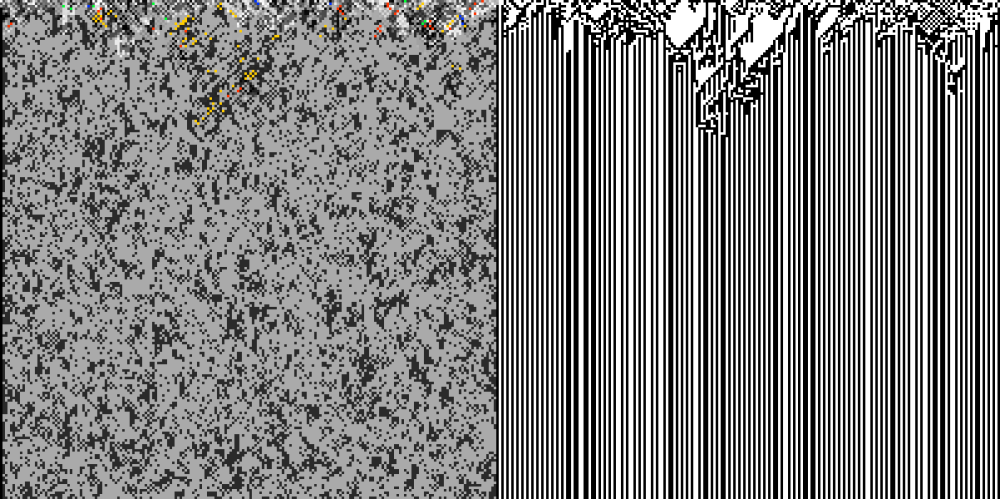
\includegraphics[width=\columnwidth]{eoc.png} 
\caption{A skewed mutation pattern \label{reef}}
\end{figure}

\subsection{2D CAs} \label{2d-results}

\textbf{[Ewen please add 1/4 to 3/4 pp. here].}

\begin{figure}
\begin{center}
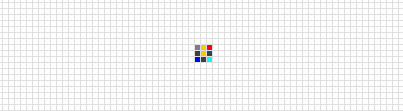
\includegraphics[width=\columnwidth]{initial2d.jpg}
(A)\\ \medskip
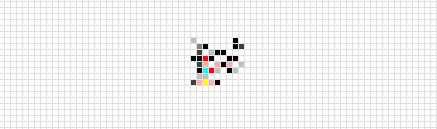
\includegraphics[width=\columnwidth]{3002d.jpg}
(B)\\ \medskip
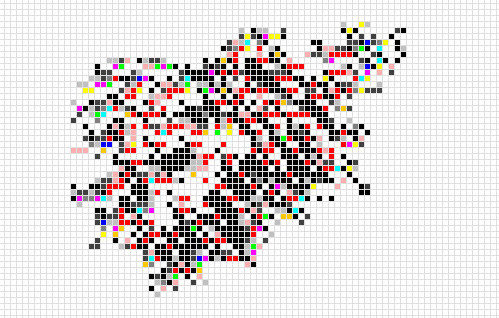
\includegraphics[width=\columnwidth]{30002d.jpg}
(C)\\ \medskip
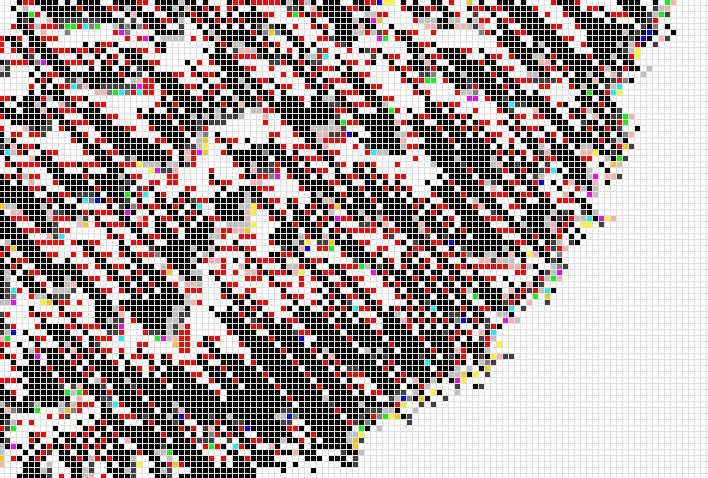
\includegraphics[width=\columnwidth]{300002d.jpg}
(D)\\
\end{center}
\caption{Two dimensional cellular automaton built using blending
  dynamics: (A) Initial state; (B-D) Evolution over time}
\end{figure}

\newpage

\section{Discussion}

The early experiments seemed to provide visual evidence that blending
is very useful: Figure \ref{metaca-taster} was much more interesting
than Figure \ref{barcode}.  The blending rule seems itself to be a
thought-provoking blend of two very different kinds of ``ethics.''
Specifically, blending seems to introduce a dynamic similar to Carol
Gilligan's \emph{ethic of care} \cite{gilligan1982different}, which
seeks to defend the relationships that obtain in a given situation.
Here this is manifested by the question ``Have my neighbours already
formed a consensus?''  This behaviour augments and extends the local
rule, which would correspond to Lawrence Kohlberg’s \emph{ethic of
  justice} (cf. \cite{benhabib1985generalized}).

However, as we saw in Section \ref{1d-results}, we would have to work
harder to find meta-rules that give rise to an ``intelligent
universe'' or in which life (considered as symbolic computation) plays
an obvious negentropic role, \emph{apr\`es} Bergson
\cite{bergson1912creative}.

One strategy that has not been fully exploited here would be to make
use of a ``Baldwin effect''
\cite{baldwin-effect,deacon2003hierarchic}, to use ``learning''
(considered as entropy) in the phenotype layer to drive evolution.
More specifically, \boxed{0\mystrut}\boxed{0\mystrut}\boxed{0\mystrut}
$\mapsto$ \boxed{0\mystrut} and
\boxed{1\mystrut}\boxed{1\mystrut}\boxed{1\mystrut} $\mapsto$
\boxed{1\mystrut} seem to be relatively uninteresting behaviours, but
they are also hard to resist under the blending dynamics as we've
defined them (compare Figures \ref{flag} and \ref{seti}).  Can we find
ways to select against them?

One observes that under our blending rule, these behaviours tend to
selected for, not against, because they are examples of the
``neighbours match'' condition.  Indeed, reviewing the essential
features of blending in the 1D case, we can use our basic principles

\begin{quote}
 \emph{If neighbours match:} \emph{then use their shared value as the result.}\\
 \emph{If neighbours don't match:} \emph{then use local logic to get the result.}
\end{quote}

\noindent to define a 1D CA rule, if we interpret ``local logic'' to
mean ``substitute my own value as the result.''  Here's how we would
then define blending for triplets:

\lstset{
  xleftmargin=.2\columnwidth, xrightmargin=.01\columnwidth
}

\begin{lstlisting}[mathescape]
0 0 0 $\mapsto$ 0    $\text{\emph{Neighbours match}}$
0 0 1 $\mapsto$ 0    $\text{\emph{Local logic}}$
0 1 0 $\mapsto$ 0    $\text{\emph{Neighbours match}}$
0 1 1 $\mapsto$ 1    $\text{\emph{Local logic}}$
1 0 0 $\mapsto$ 0    $\text{\emph{Local logic}}$
1 0 1 $\mapsto$ 1    $\text{\emph{Neighbours match}}$
1 1 0 $\mapsto$ 1    $\text{\emph{Local logic}}$
1 1 1 $\mapsto$ 1    $\text{\emph{Neighbours match}}$
\end{lstlisting}

This is Wolfram's Rule 23: and as it happens, its evolutionary
behaviour is not particularly interesting.  Of course, for blending at
the genotype level, ``local logic'' can be determined by any CA.  Even
so, when we use blending bitwise on alleles, we only ever run the
local logic on half of the cases, and moreover it always the same
half, determined by a ``censored'' version of Rule 23.

\begin{lstlisting}[mathescape]
0 0 0 $\mapsto$ 0    $\text{\emph{Neighbours match}}$
0 0 1 $\mapsto$ *    $\text{\emph{Local logic}}$
0 1 0 $\mapsto$ 0    $\text{\emph{Neighbours match}}$
0 1 1 $\mapsto$ *    $\text{\emph{Local logic}}$
1 0 0 $\mapsto$ *    $\text{\emph{Local logic}}$
1 0 1 $\mapsto$ 1    $\text{\emph{Neighbours match}}$
1 1 0 $\mapsto$ *    $\text{\emph{Local logic}}$
1 1 1 $\mapsto$ 1    $\text{\emph{Neighbours match}}$
\end{lstlisting}

Rather than using Censored Rule 23 as our template, we could instead
have the template determined by phenotype data, thereby inserting the
phenotype as a ``hidden layer'' in the computation.

The standard template could be understood to be generated by locking in
%
\boxed{0\mystrut}\boxed{0\mystrut}\boxed{0\mystrut} $\mapsto$ \boxed{0\mystrut}
%
along with a ``variation''\footnote{%
%
\boxed{0\mystrut}\boxed{1\mystrut}\boxed{0\mystrut} =
%
\boxed{0\mystrut}\boxed{0\mystrut}\boxed{0\mystrut} +
%
\boxed{\:\:\:\mystrut}\boxed{1\mystrut}\boxed{\:\:\:\mystrut}}
%%
\boxed{0\mystrut}\boxed{1\mystrut}\boxed{0\mystrut} $\mapsto$
\boxed{0\mystrut} and the bitwise inverses of these.  A wider class of
templates could calculated from arbitrary phenotype data by the same
operations.  What we would lose in abandoning the intuition associated
with local blending, we may be repayed through a much more abstract
but richer procedural blend, operating at the level of
genotype+phenotype evolution.  At the very least, we can point to a
generic space, namely the locked-in local rule which would be carried
over (along with its variants) from the phenotype to the corresponding
alleles.

This sort of system co-evolution has been understood to be relevant
from both a philosophical \cite{mead1932philosophy} and empirical
perspective \cite{van1973new}.  It presents a fertile ground for
further computational research.

\section{Conclusion}
% Some of the relevant references are below.
%% \nocite{*}
%% We have considerably advanced the field of research.  But much remains
%% to be done.  We can start by checking which references we actually
%% use, and removing the \verb|\nocite{*}| command from this section.

This research was inspired by the aim to build an example of
computational blending that matched, to some extent, the way blending
might work in social settings.  One person suggests an idea, and
another offers a variant of that, a third brings in another idea from
elsewhere and some combination is made.  The next day, things head in
another direction completely.  Our progress in this research project
has followed this sort of trajectory: from an initial critique of
blending theory (``it's not dynamic enough!'') to some tentative
examples showing how large-scale system dynamics can be driven by
local behaviour in an emergent manner.  Perhaps the most exciting
interesting aspect of this research is the relationship between these
emergent dynamics and the meta-rules.  Whereas previous CA research
has shown that complex global behaviour can be generated from a set of
simple, local rules, this project gives an enticing glimpse of a
future research programme that carries out a computational search for
those very rules (out of the many possible) that lead to system
behaviour we would recognize as ``intelligent.''

\section{Acknowledgements}

Coinvent, etc.

\bibliography{metaca}

\end{document}
